\documentclass[aspectratio=1610]{beamer}
%\linespread{1.5}\selectfont
\usepackage{graphicx}
\usepackage{booktabs}
\usepackage{siunitx}
\usepackage{dcolumn}
\usepackage{float}
\usepackage{placeins}
\usepackage{lscape} 
\usepackage{tikz}
\usepackage[export]{adjustbox}
\usepackage{ragged2e}
\usepackage{centernot}
\setcounter{tocdepth}{2}
\justifying
\usepackage{outlines}
\usepackage{amsmath}
\usepackage{booktabs}
\usepackage{float}
\usepackage{dcolumn}
\usepackage{longtable}
\usepackage{array}
\usepackage{multirow}
\usepackage{wrapfig}
\usepackage{float}
\usepackage{colortbl}
\usepackage{pdflscape}
\usepackage{multirow}
\usepackage{graphicx}
\usepackage{tabu}
\usepackage{threeparttable}
\usepackage{caption}
%\captionsetup{labelformat=empty}
%\captionsetup{font=footnotesize}
\usepackage{subcaption}
\usepackage{threeparttable}
\usepackage[normalem]{ulem}
\usepackage{makecell}
\usepackage{xcolor}
\usepackage{hyperref}
\hypersetup{
    colorlinks = true, 
    linkcolor = red, 
    urlcolor = teal, 
    citecolor = blue}

%\usepackage{caption}
%\captionsetup{labelformat=empty}
\usepackage{appendixnumberbeamer}
\renewcommand{\raggedright}{\leftskip=0pt \rightskip=20pt plus 0cm}

\DeclareUnicodeCharacter{0301}{\'{e}}
\DeclareUnicodeCharacter{2212}{-}
\DeclareUnicodeCharacter{0327}{\c}

\usepackage[backend = biber, style=authoryear, sorting = nty, maxcitenames=1]{biblatex}

\addbibresource{citations_sesmarias.bib}

\graphicspath{{~/OneDrive - University of Illinois - Urbana/Research/Projects/Sesmarias Brazil/Figures/Descriptive/}}

%\addbibresource[location = remote]{https://raw.githubusercontent.com/ViniOkadaSilva/Papers/master/Sesmarias/citations_sesmarias.bib}

\DeclareFieldFormat{citehyperref}{%
  \DeclareFieldAlias{bibhyperref}{noformat}% Avoid nested links
  \bibhyperref{#1}}

\DeclareFieldFormat{textcitehyperref}{%
  \DeclareFieldAlias{bibhyperref}{noformat}% Avoid nested links
  \bibhyperref{%
    #1%
    \ifbool{cbx:parens}
      {\bibcloseparen\global\boolfalse{cbx:parens}}
      {}}}

\savebibmacro{cite}
\savebibmacro{textcite}

\renewbibmacro*{cite}{%
  \printtext[citehyperref]{%
    \restorebibmacro{cite}%
    \usebibmacro{cite}}}

\renewbibmacro*{textcite}{%
  \ifboolexpr{
    ( not test {\iffieldundef{prenote}} and
      test {\ifnumequal{\value{citecount}}{1}} )
    or
    ( not test {\iffieldundef{postnote}} and
      test {\ifnumequal{\value{citecount}}{\value{citetotal}}} )
  }
    {\DeclareFieldAlias{textcitehyperref}{noformat}}
    {}%
  \printtext[textcitehyperref]{%
    \restorebibmacro{textcite}%
    \usebibmacro{textcite}}}

\renewcommand*{\nameyeardelim}{\addcomma\space}

\mode<presentation>
{
  \usefonttheme{default}  % or try serif, structurebold, ...
  \setbeamertemplate{page number in head/foot}{}
  \setbeamertemplate{navigation symbols}{}
  \setbeamertemplate{caption}[numbered]
    \setbeamertemplate{footline}{}
}

\usepackage{setspace}
\usepackage{graphicx}

\newcommand{\tinytable}[1]{\textcolor{black}{\tiny \input{#1}}}

\graphicspath{{~/OneDrive - University of Illinois - Urbana/Research/Writing/git/Sesmarias/Pictures/}}

\beamertemplatenavigationsymbolsempty

%Information to be included in the title page:
\title{Portuguese Colonial Land Grants in Brazil: Long-term Effects on Inequality and Economic Development}
\author{Vinicius Okada da Silva}
\date{May 10th, 2024}

%\setbeamertemplate{footline}[frame number]

\begin{document}

\setbeamertemplate{itemize items}[circle]

\begin{frame}[plain, noframenumbering]
	\titlepage
\end{frame}

\AtBeginSection[]
{
  \begin{frame}<beamer>[noframenumbering,plain]
    \frametitle{Outline}
    \tableofcontents[currentsection]
  \end{frame}
}

\AtBeginSubsection[]
{
  \begin{frame}<beamer>[noframenumbering,plain]
    \frametitle{Outline}
    \tableofcontents[currentsubsection,
    sectionstyle=show/shaded,
    subsectionstyle=show/shaded]
  \end{frame}
}

\begin{frame}{Motivation}
    \begin{outline}
        \1 Inequality in access to land is a key political and economic issue in Brazil
            \vspace{2mm}
            \2 ``\textcolor{red}{\textbf{Brazil has one of the highest levels of inequality of land distribution in the world}} [...] \textcolor{red}{\textbf{An estimated 1\% of the population owns 45\% of all land in Brazil}}.'' \parencite{Usaid2016-xs}
        \vspace{2mm}
        \pause 
        \1 Large plots of land are often associated with low utilization \parencite[p.~1]{De_Oliveira_Andrade1980-xz}
        \pause 
        \vspace{2mm}
            \2 Brazilian Agrarian Reform Agency in 2010, reported that ``72\% of all land occupied by large holdings was considered unproductive''.
        \vspace{2mm}
        \pause 
        \1 Broad economic ramifications
            \vspace{2mm}
            \2 Land monopolies lead to the depression of rural wages alongside the stagnation of the consumer market \parencite[p.~1]{De_Oliveira_Andrade1980-xz}.
    \end{outline}
\end{frame}

\begin{frame}[t]{Motivation}
    \begin{outline}
        \1 Land inequality is not a recent issue \parencite{Alston2010-cn}
    \end{outline}
    \pause 

    \begin{figure}
        \centering
        \includegraphics[width = .8\paperwidth]{/Users/vinicius/Library/CloudStorage/OneDrive-UniversityofIllinois-Urbana/Research/Writing/git/Sesmarias/Pictures/gini_land.png}
    \end{figure}

    \pause 
    \begin{outline}
    \1 A report to the Minister of Agriculture in 1873 states that ``The major part of the land in our province is divided into great properties, remains of the ancient [land grants], of which few have been subdivided''\parencite[p.~325]{Smith1972-dv}
    \end{outline}
\end{frame}

\begin{frame}{Research Question}
    \begin{outline}
        \1 How much of present-day land inequality can be traced to historical land grants in Brazil?
        \vspace{2mm}
        \pause 
        % make more clear this out
    \end{outline}
    \textbf{Identification:}
    \vspace{2mm}
    \begin{enumerate}
        \item \textbf{1-1 Propensity Score Matching}
        \vspace{2mm}
        \item \textbf{Treaty of Tordesillas}: Assignment of Portuguese and Spanish Brazil until 1750. 
        \vspace{2mm}
        \item \textbf{Colonial Policy Variation}: Coastal Ban on Livestock within 80km in 1701
        \vspace{2mm}
        \item \textbf{Instrumental Variable in the Southeast}: Explorer Routes in the Southeast.
    \end{enumerate}
    \pause 
    \vspace{2mm}
    $\Rightarrow$ \textcolor{red}{\textbf{Main Takeaway}}: All methods point toward a significant increase in 1995 land concentration in municipalities that had a grant.
\end{frame}

\begin{frame}{Contribution}
    \begin{outline}
        \1 Novel dataset on the distribution of colonial grants in Brazil.
        \vspace{2mm}
        \1 First to study and document the long-term effects of colonial land distribution on the present in Brazil.
        \vspace{2mm}
            \2 Americas: 
            \cite{Wigton-Jones2020-ex} (JEG),
            \cite{Sellars2018-yp} (JDE),
            \cite{Smith2023-ip} (WP)
            \vspace{2mm}
            \2 India and Africa: 
            \cites{Banerjee2005-ki} (AER)
        \vspace{2mm}
        \1 Understand the persistent effects of colonial Brazil's economic structure on the present.
        \vspace{2mm}
        \2 Institutional and Natural Endowments: 
        \cite{Acemoglu2001-dz} (AER), 
        \cite{Sokoloff2000-mb} (JEP).
        \vspace{2mm}
        \2 
        \cite{Naritomi2012-or} (JEH), 
        \cite{Musacchio2014-pq} (JEH),
        \cite{Laudares2022-vy} (WP). 
    \end{outline}
\end{frame}

% Maybe organize everything to be methods all at once vs. add keys and pre- post-1700
% Identification and then challenge - be clear on year vs. state balanced..
% Take a look if there's somewhere on the total number of grants.
% Moves the challenges to identification make smaller points - How many municipalities only have a single grant, there could bias results.
% How many of the possible treat to non-treat could work. - in most cases 

\section{Background}

\begin{frame}{Background}{Law Origins}
    \begin{outline}
        \1 Originally, the \textit{sesmarias} (land grants) were used as a land distribution policy created in Portugal to deal with the allocation of land post-Black Death.
        \vspace{2mm}
        \1 Granted small holdings to help repopulate and drive economic growth in affected regions.
    \end{outline}
\end{frame}

\begin{frame}{Background}{In Brazil}
    \begin{outline}
        \1 Goal was to encourage Portuguese settlement in Brazil.
        \vspace{2mm}
            \2 Reason on why they were much larger than in Portugal.
        \vspace{2mm}
        \1 One of the few ways to have access to land in colonial Brazil and given to people who could afford to develop the land \parencites{Smith1944-oi}{Dean1971-iq}.
        \vspace{-1mm}
        \1 People without direct access to it were often marginalized \parencite{Simonsen2005-ps}.
        \vspace{2mm}
        \1 Lasted until 1822.
    \end{outline}    
\end{frame}

\begin{frame}{Background}{Procedure}
    \begin{outline}
        \1 Petitioner submits a letter for an unoccupied land detailing their qualifications (captain, governor, etc.)
        \vspace{2mm}
        \1 Governor reads it, and if accepted returns back a letter with the requirements for the petitioner to satisfy.
        \vspace{2mm}
        \1 Five years to develop the land
        \vspace{2mm}
        \1 If successful, upon an inspection, the land was legally transferred from the government to the petitioner.
        \vspace{2mm}
        \1 Able to sell, pass down as inheritance, etc. 
    \end{outline}
\end{frame}

%\begin{frame}{Application Procedure}
%    [add nice little animation here]
%\end{frame}

\begin{frame}{Background}{Persistence}
    \begin{outline}
        \1 In 1850, the Land Law was passed, dictating how land was to be distributed in post-independence Brazil.
        \vspace{2mm}
            \2 Decided by large landowners, consolidated the land access in their hands.
        \vspace{2mm}
        \1 Historical and anecdotal evidence of the land grants having permanent effects in Brazilian economic structure:
        \vspace{2mm}
            \2 Early studies argued it led to the development of the ``\textcolor{red}{\textbf{economic aristocracy of the colonial society}}'' and the ``\textcolor{red}{\textbf{principal cause of the [large estates]}}'' in Brazil \parencites[p.~36]{Lima1954-td}[p.~48]{Da_Costa_Porto1979-dz}. 
    \end{outline}
\end{frame}

%\begin{frame}{Channels}
%    \begin{outline}
%        \1 \textbf{Labor Outcomes} $\Rightarrow$ Land distribution could lead to different specialization (sugarcane vs. livestock).
%        \pause 
%        \vspace{2mm}
%        \1 \textbf{Land Tenure} $\Rightarrow$ Different sizes of land grants could lead to different utilization of land, and how owners would exploit it.
%        \pause 
%        \vspace{2mm}
%        \1 \textbf{Demographic Differences} $\Rightarrow$ Land grants often required African slaves, which could skew the demographics of a location.
%    \end{outline}
%\end{frame}

%\begin{frame}{Identification Strategy}
%    \begin{outline}
%        \1 
%        \1 IV
%        \1 Coastal Ban on Livestock
%    \end{outline}
%\end{frame}

\section{Data}

\begin{frame}{Data}
    \begin{outline}
        \1 Land Grant Locations:
        \vspace{2mm}
            \2 Information on the land grants from the \href{http://plataformasilb.cchla.ufrn.br/}{Sesmarias of the Luso-Brazilian Empire Database} and my own archival work [\textbf{Novel Data}]
    \end{outline}
\end{frame}

\begin{frame}[t]
    {\hypertarget{manuscripts}Land Grant Dataset}
    Three main types of documents used:
    \only<1>{
        \begin{enumerate}
            \item Manuscript Only (Northeast)
        \end{enumerate}

        \begin{figure}[htbp]
            \begin{center}
            \label{fig:example_letter_other}
            \begin{subfigure}[b]{0.35\textwidth}
            \centering
            \vspace{-20cm}
            \includegraphics[width = \textwidth]
            {~/OneDrive - University of Illinois - Urbana/Research/Writing/git/Sesmarias/Pictures/0167f614a7c3b3fd38127f1545dbee7c.pdf}
            \end{subfigure}
            \begin{subfigure}[b]{0.35\textwidth}
            \centering
            %\vspace{-7.4cm}
            \includegraphics[page = 1, width = \textwidth]
            {~/OneDrive - University of Illinois - Urbana/Research/Writing/git/Sesmarias/Pictures/ea71ea6ac7c5ec3cefa24ded60ac6438.pdf}
            \end{subfigure}
            \end{center}
          \end{figure}
    }

    \only<2>{
        \begin{enumerate}
            \setcounter{enumi}{1}
            \item Digitized Manuscript (Sao Paulo):
        \end{enumerate}
        \begin{figure}[h!]
            \begin{center}
            \label{fig:example_letter_sp}
            \vspace{3mm}
            \makebox[\textwidth]	
            {\includegraphics[width = 0.35\textwidth]{~/OneDrive - University of Illinois - Urbana/Research/Projects/Sesmarias Brazil/Documents/Sao Paulo/example.png}}
            \end{center}
        \end{figure}
    }

    \only<3>{
        \begin{enumerate}
            \setcounter{enumi}{2}
            \item Inventory (Minas Gerais):
        \end{enumerate}
        \begin{figure}[htbp]
            \begin{center}
              \vspace{3mm}
              \makebox[\textwidth]	
              {\includegraphics[width = 0.75\textwidth]{~/OneDrive - University of Illinois - Urbana/Research/Writing/git/Sesmarias/Pictures/minas_inventory.png}}
              \end{center}
          \end{figure}
    }
\end{frame}

\begin{frame}{Georeferencing Example}
    \only<1>
    {
        \begin{columns}
            \begin{column}{0.5\textwidth}
                \begin{figure}[h!]
                    \begin{center}
                    \vspace{3mm}
                    \makebox[\textwidth]	
                    {\includegraphics[width = \textwidth]{~/OneDrive - University of Illinois - Urbana/Research/Writing/git/Sesmarias/GR_Pics/text.png}}
                    \end{center}
                \end{figure}
            \end{column}

            \begin{column}{0.5\textwidth}
                \begin{itemize}
                    \item \textbf{Four geographical markers}: \textit{Campos de Ytacurubitiva} (Fields of Ytacurubitiva), Boigi Mirim,  Rio Grande de Anhemby, and Rio Guyao
                \end{itemize}
            \end{column}
        \end{columns}
    }

    \only<2-5>
    {
        \begin{columns}
            \begin{column}{0.5\textwidth}
                \begin{figure}[h!]
                    \begin{center}
                    \vspace{3mm}
                    \makebox[\textwidth]	
                    {\includegraphics[width = \textwidth]{~/OneDrive - University of Illinois - Urbana/Research/Writing/git/Sesmarias/GR_Pics/text.png}}
                    \end{center}
                \end{figure}
            \end{column}

            \begin{column}{0.5\textwidth}
                \begin{itemize}
                    \item<2-5> \textit{Campos de Ytacurubitiva} (Fields of Ytacurubitiva) $\rightarrow$ Same as Itaquaquecetuba (Costa, 2021).
                    \item<3-5> Boigi Mirim $\rightarrow$ Municipality of Mogi das Cruzes (Leme, 2014).
                    \item<4-5> Rio Grande de Anhemby $\rightarrow$ Tiete River (Vilardaga, 2020).
                    \item<5-5> Rio Guyao $\rightarrow$ Guaio River.
                \end{itemize}
            \end{column}
        \end{columns}
    }

    \only<6>
    {
        \begin{figure}[h!]
            \begin{center}
            \vspace{3mm}
            \makebox[\textwidth]	
            {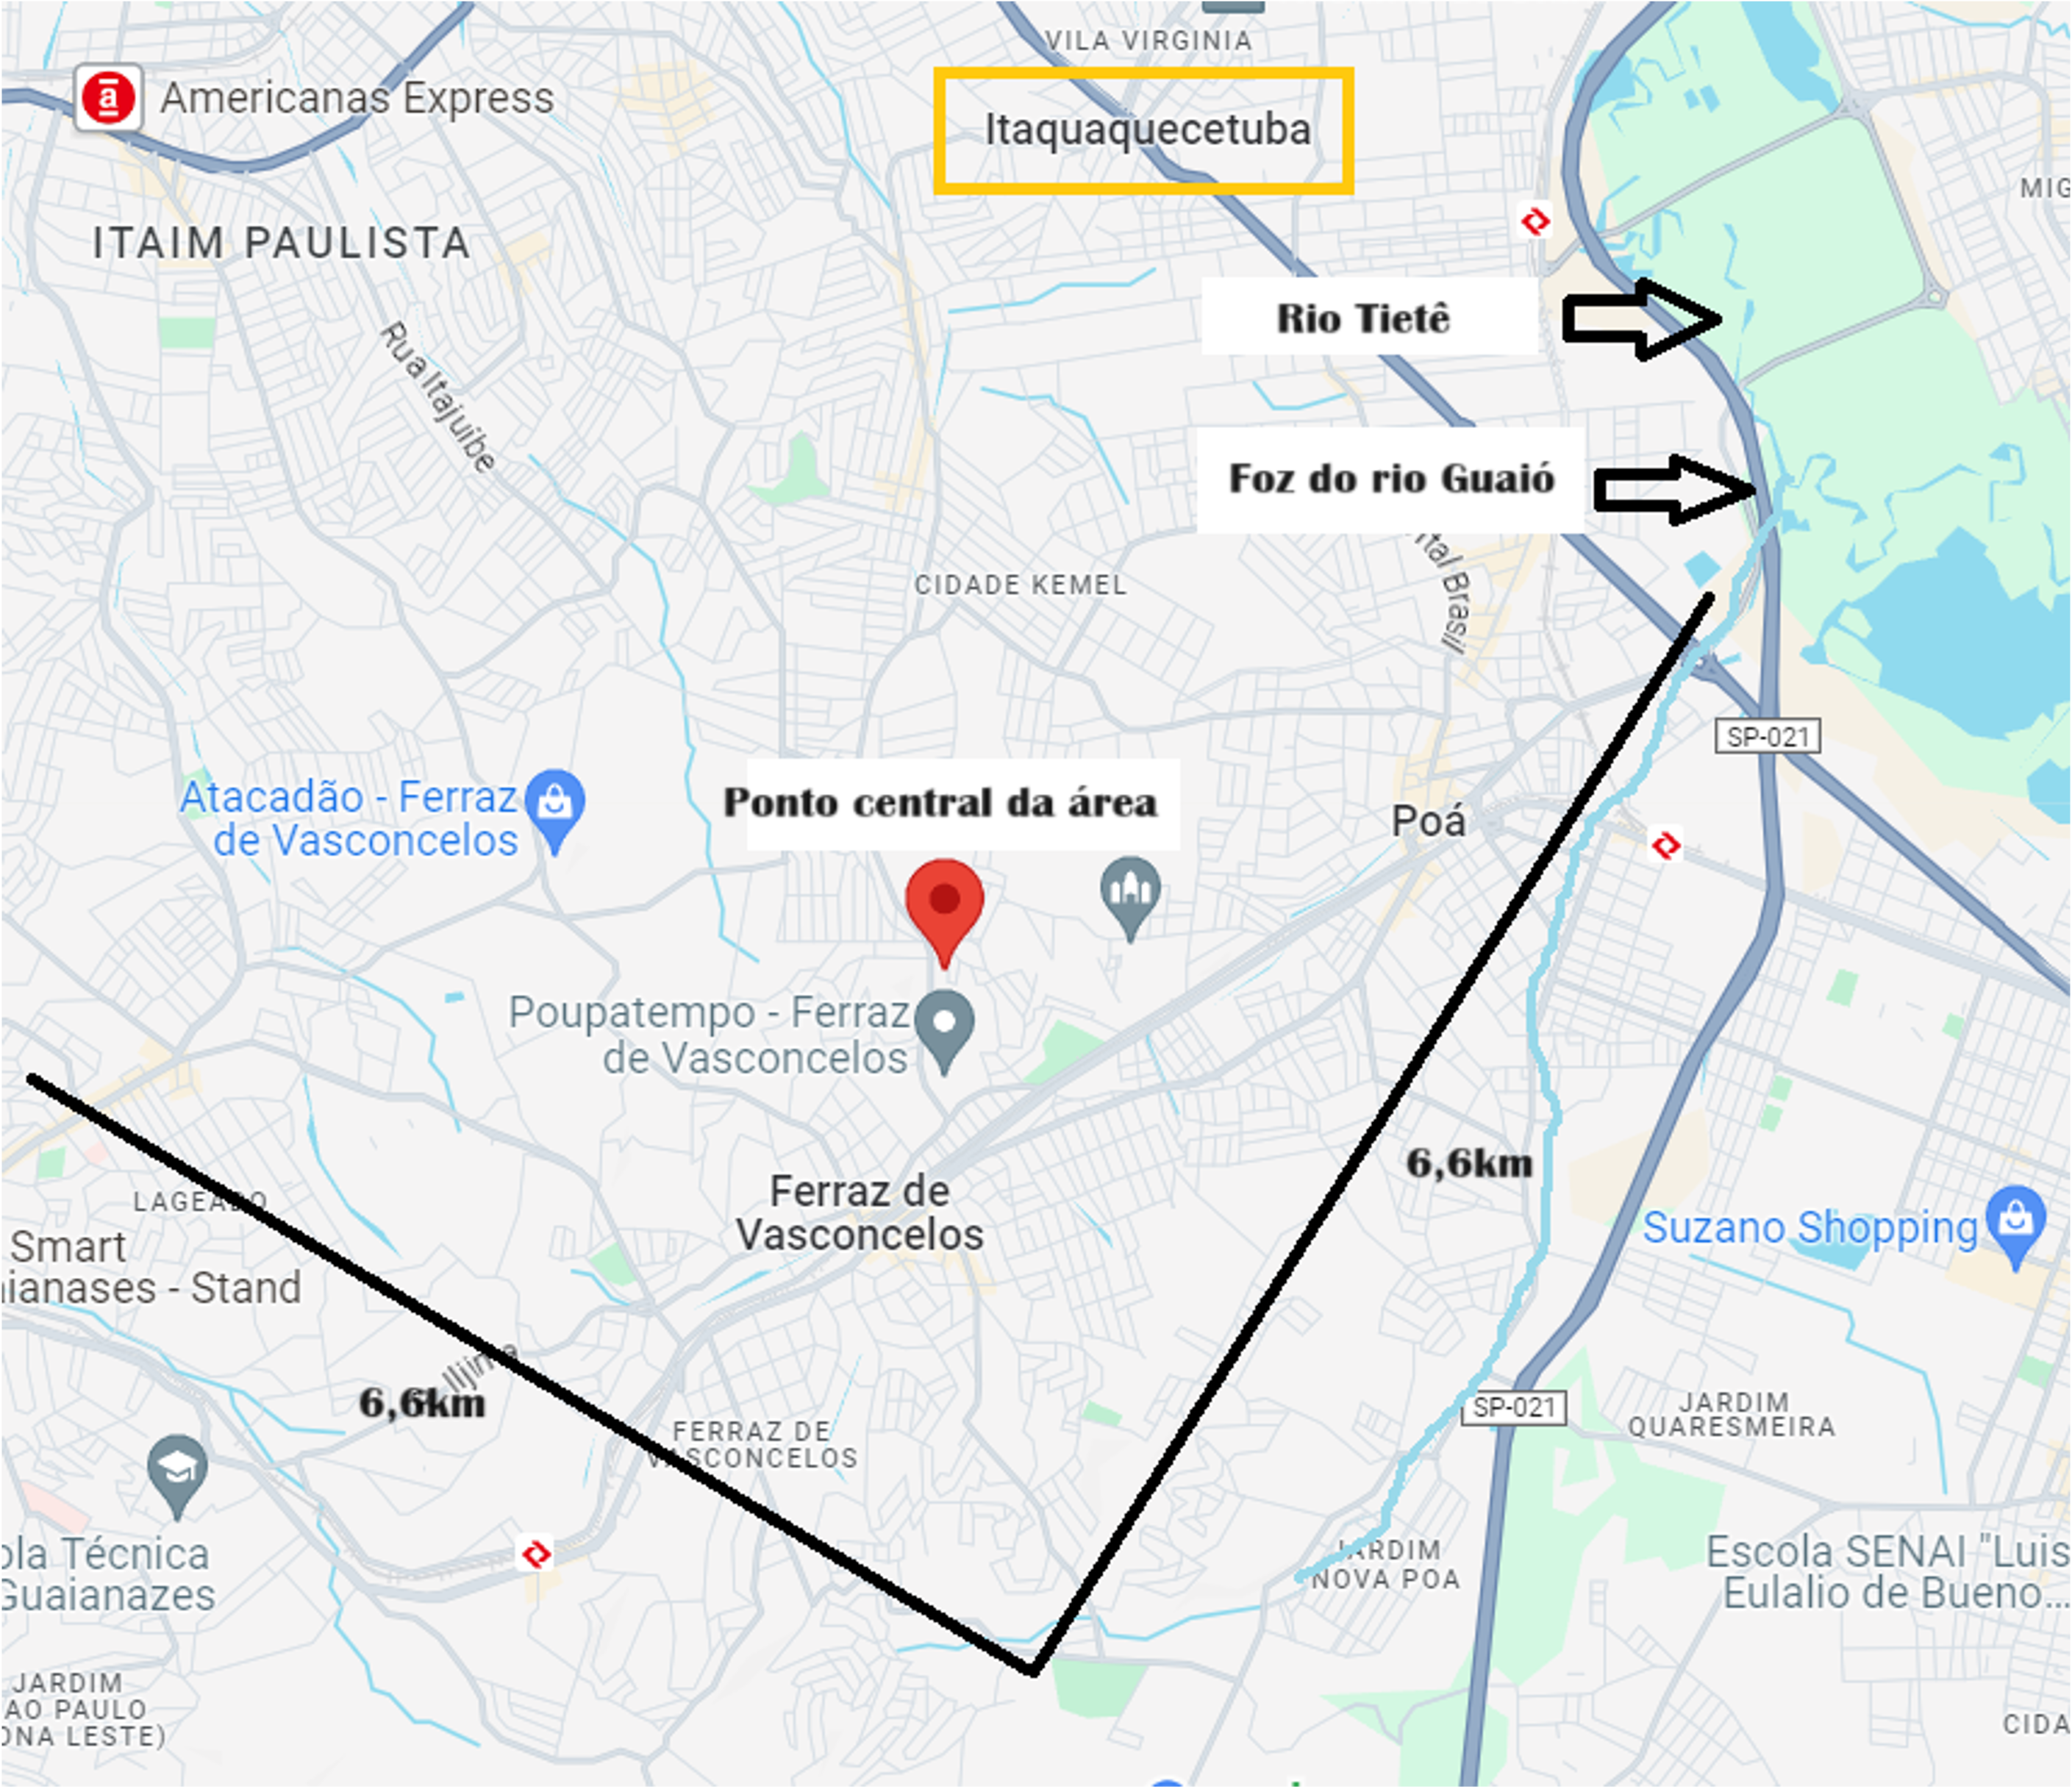
\includegraphics[width = 0.55\textwidth]{~/OneDrive - University of Illinois - Urbana/Research/Writing/git/Sesmarias/GR_Pics/georeferencing.png}}
            \end{center}
        \end{figure}  

        \centering
        \textbf{Coordinates:} -46.3, -23.5
    }

\end{frame}

\begin{frame}{Full Land Grant Dataset}
    \begin{figure}[h!]
        \begin{center}
           \makebox[\textwidth]			 
           {\includegraphics[width=\textwidth]{/Users/vinicius/Library/CloudStorage/OneDrive-UniversityofIllinois-Urbana/Research/Projects/JMP/02. Figures/00.Maps/land_grants_distribution_1991.png}}
        \end{center}
      \end{figure}
    %add button here zooming in to the Northeast specifically to show there is variation
\end{frame}

\begin{frame}{Data Assumptions}
    \only<1>{
        \begin{enumerate}
            \item Sample Selection:
        \end{enumerate}
        \vspace{2mm}
        \hspace{3mm} - Data only contains land grants that were able to be georeferenced \textbf{and} saved in archives.
        \vspace{2mm}
        \begin{outline}
            \1 Assume that the dataset is at least partially \textbf{representative} of all the grants 
            %[table here showing the match by state, time period][add ref here for an example of a letter that could not be read]
        \end{outline}
    }

    \only<2>{
        \begin{enumerate}
            \setcounter{enumi}{1}
            \item Geolocation Procedure:
        \end{enumerate}
        \vspace{2mm}
        \hspace{3mm} - Treatment assignment could vary on how well the georeferencing is done.
        \vspace{2mm}
        \begin{outline}
            \1 Described previously.
            \vspace{2mm}
            \1 Uses a variety of historical, and scholarly work.
            \vspace{2mm}
            \1 \textbf{Last resort}: pinpoint to the nearest municipality.
        \end{outline}
    }
\end{frame}

\begin{frame}{\hypertarget{data}Data}
    \begin{outline}
        \1 Land Grant Locations:
        \vspace{2mm}
            \2 Information on the land grants from the \href{http://plataformasilb.cchla.ufrn.br/}{Sesmarias of the Luso-Brazilian Empire Database}  and my own archival work [\textbf{Novel Data}] 
            \hyperlink{year_dist}{\beamerbutton{Grant by Decade Distribution}}
        \vspace{2mm}
        \1 Present-Day Effects on Land Inequality (1995 Municipalities)
        \vspace{2mm}
            \2 1995 Brazilian Agricultural Census
            \vspace{2mm}
            \2 \textcolor{red}{\textbf{Measure of inequality}}: \% of Total Agricultural Land in a Municipality that is in establishments of over 2,000 ha (20 $km^2$ or 4,912 acres).
            \pause
            \vspace{2mm}
            \2 For reference the UIUC campus is 6,370 acres.
        \vspace{2mm}
        %\1 Check whether they had an effect in the past:

        %\1 Present-Day Effects on Land Usage (10 x 10km Grid)
        %\vspace{2mm}
        %    \2 1985 LandSat data from MapBiomas
        %\vspace{2mm}
    \end{outline}
\end{frame}

\section{Identification Strategies}

\begin{frame}{Identification Strategy I}{Matching}

    \begin{equation}
        LandGrant_m = X_{m} + \mu_s + \epsilon_{m,s}
    \end{equation}
    \vspace{2mm}
    \begin{outline}
        \1 Variables used to match: latitude, longitude, mean elevation, mean slope, soil quality for food crops \parencite{Galor2016-ba}, potential sugarcane output from the FAO, the distance to the coast, distance to the nearest river, and the presence of four types of soil. 
        \vspace{2mm}
            \2 All important geographical measures of settler presence.
        \vspace{2mm}
        \1 Estimate the coefficients on the $X_m$ $\rightarrow$ predicts the propensity score that a municipality received a grant.
        \vspace{2mm}
        \1 1-1 Nearest Neighbor Matching: an untreated municipality is assigned as a control for a treated municipality.
        \vspace{2mm}
        \1 Generates the \textbf{matched sample} of municipalities.
    \end{outline}   
\end{frame}

\begin{frame}{\hypertarget{matching} Identification Strategy I}{Matching}

    For both the matched and unmatched samples:

    \begin{equation}
        Y_{m,s} = LandGrant_m + X_{m} + \mu_s + \epsilon_{m,s}
    \end{equation}
    \begin{outline}
        \1 \textbf{Key Assumption}: Untreated municipalities are similar in both observables and unobservables as treated municipalities. \hyperlink{propensity_score}{\beamerbutton{Propensity Score Overlap}}
        \vspace{2mm}
        \1 Further exploit variation on 1698 law that limited grant size.
    \end{outline}

    \begin{equation}
        Y_{m,s} = \gamma_1 \cdot Pre1700Grant_m + \gamma_2 \cdot Post1700Grant_m + X_{m} + \mu_s + \epsilon_{m,s}
    \end{equation}
\end{frame}

\begin{frame}{Identification Strategy II}{Tordesillas Treaty}
    \begin{outline}
        \1 Brazil was split between Portuguese and Spanish sides in 1494 (before the first Europeans arrived in Brazil).
        \vspace{2mm}
        \1 By law lasted until 1750.
        \vspace{2mm}
        \1 Generates variation in where the grants \textbf{could be assigned}, and the \textbf{exposure of two colonization types}.
        \vspace{2mm}   
            \2 Spanish side was not deeply settled, few cities, and some missionary activity \parencite{Barsanetti2021-hp}.
        \vspace{2mm}   
        \1 Focused only on the Southeastern states of Sao Paulo and Minas Gerais - both have municipalities on either side of the treaty line.
    \end{outline}
\end{frame}

\begin{frame}[t]{Identification Strategy II}{Tordesillas Treaty}
    \begin{equation*}
        \begin{split}
        Y_{m,s} = & \beta_1 \cdot (Grant_m  * Portuguese_m) + \beta_2 \cdot (Grant_m * Spanish_m) + \\
        & \delta \cdot  Portuguese_m + X_{m} + \mu_s + \epsilon_{m,s}
        \end{split}
    \end{equation*}
    \begin{outline}
        \1 Follow \textcite{Laudares2022-vy} to define the Tordesillas Treaty at 48.7 W. 
        \vspace{2mm}
        \1 Test historical predictions
        \vspace{2mm}
        \1 \textbf{Control Group:} Municipalities on the \textcolor{red}{\textbf{Spanish Side}} that \textcolor{red}{\textbf{did not}} receive a grant.
        \vspace{2mm}
            \2 $X_m$ same as previous specifications + \textbf{distance to the line}.
        \vspace{2mm}
            \2 $\mu_s$ state fixed effects.
    \end{outline}
\end{frame}

\begin{frame}{Identification Strategy II}{Tordesillas Treaty}
    \begin{figure}[h!]
        \begin{center}
           \makebox[\textwidth]			 
           {\includegraphics[width=0.75\paperwidth]{/Users/vinicius/Library/CloudStorage/OneDrive-UniversityofIllinois-Urbana/Research/Projects/JMP/02. Figures/00.Maps/sesmarias_tordesillas.png}}
        \end{center}
      \end{figure}
\end{frame}

\begin{frame}[t]{Identification Strategy II}{Hypothesis and Predictions}
    \begin{equation*}
        \begin{split}
        Y_{m,s} = & \beta_1 \cdot (Grant_m  * Portuguese_m) + \beta_2 \cdot (Grant_m * Spanish_m) + \\
        & \delta \cdot  Portuguese_m + X_{m} + \mu_s + \epsilon_{m,s}
        \end{split}
    \end{equation*}
    \begin{table}[]
    \centering
    \resizebox{0.75\textwidth}{!}{%
    \begin{tabular}{|c|l|c|}
    \hline
    \multicolumn{1}{|l|}{\textbf{Coefficients}} & \textbf{If the Following is True}                                                                                                                    & \multicolumn{1}{l|}{\textbf{Predicted Sign}} \\ \hline
    $\delta$                                    & \begin{tabular}[c]{@{}l@{}}Portuguese colonization led to\\ \textbf{increase} in land inequality \\ relatively to Spanish colonization.\end{tabular} & +                                            \\ \hline
    $\beta_1$                                   & \multirow{2}{*}{\begin{tabular}[c]{@{}l@{}}The land grants led to \\ land inequality.\end{tabular}}                                           & +                                            \\ \cline{1-1} \cline{3-3} 
    $\beta_2$                                   &                                                                                                                                                      & +                                            \\ \hline
    \end{tabular}%
    }
    \end{table}
\end{frame}

\begin{frame}{Identification Strategy III}{Coastal Ban on Livestock}
    \begin{outline}
        \1 In 1701, a Royal Decree was established banning livestock raising within 80km of the coast \parencites[p~.40]{Fausto2014-bh}[p~.198]{Simonsen2005-ps}[p~.460]{Bethell1984-of}.
        \vspace{2mm}
            \2 The main reason was that livestock was destroying the crops being planted on the coast.
        \vspace{2mm}
        \pause 
        \1 Generates variation on the \textbf{grant locations} and \textbf{possible economic activity}.
        \vspace{-1mm}
            \2 The law led to ``a clear specialization between the two activities'' \parencite{Ribeiro2012-lb}.
        \1 Livestock grants are often associated with large estates, since cattle needed the area to roam \parencite[p~.41]{Fausto2014-bh}.
    \end{outline}
\end{frame}

\begin{frame}[t]{Identification Strategy III}{Coastal Ban on Livestock}
    \begin{equation*}
        \begin{split}
        Y_{m,s} = & \beta_1 \cdot (Pre1700Grant_m  * More80km_m) + \beta_2 \cdot (Pre1700Grant_m * Less80km_m) + \\  
        & \delta \cdot  More80km_m + X_{m} + \mu_s + \epsilon_{m,s}
        \end{split}	
      \end{equation*}

      \begin{equation*}
        \begin{split}
        Y_{m,s} = & \zeta_1 \cdot (Post1700Grant_m  * More80km_m) + \zeta_2 \cdot (Post1700Grant_m * Less80km_m) + \\ 
        & \delta \cdot  More80km_m + X_{m} + \mu_s + \epsilon_{m,s}
        \end{split}
      \end{equation*}
    
    \begin{outline}
        \1 \textbf{Control Group:} Municipalities within 80km of the coast that \textcolor{red}{\textbf{did not receive a grant}}
        \vspace{2mm}
        \1 First test whether there is an increase in the \textbf{percentage of agricultural area used for livestock}.
    \end{outline}
\end{frame}

\begin{frame}[t]{Identification Strategy III}{Coastal Ban on Livestock}
    \begin{equation*}
        \begin{split}
        Y_{m,s} = & \beta_1 \cdot (Pre1700Grant_m  * More80km_m) + \beta_2 \cdot (Pre1700Grant_m * Less80km_m) + \\  
        & \delta \cdot  More80km_m + X_{m} + \mu_s + \epsilon_{m,s}
        \end{split}	
      \end{equation*}
      \begin{equation*}
        \begin{split}
        Y_{m,s} = & \zeta_1 \cdot (Post1700Grant_m  * More80km_m) + \zeta_2 \cdot (Post1700Grant_m * Less80km_m) + \\ 
        & \delta \cdot  More80km_m + X_{m} + \mu_s + \epsilon_{m,s}
        \end{split}
      \end{equation*}

\only<1>{
\begin{table}[]
    \centering
    \resizebox{\textwidth}{!}{%
    \begin{tabular}{|c|c|c|c|}
    \hline
    \textbf{Coefficients}                                       & \textbf{If following is True}                                                                                                                                           & \textbf{Effects on Livestock} & \textbf{Effects on Land Inequality} \\ \hline
    \begin{tabular}[c]{@{}c@{}}\\\\ $\beta_1$\\ \\\end{tabular} & \multirow{2}{*}{\begin{tabular}[c]{@{}c@{}}Expansion of cattle towards the West\\ was driven by the grants and livestock\\ required larger plots of land.\end{tabular}} & $\sim$                        & + or 0                              \\ \cline{1-1} \cline{3-4} 
    \begin{tabular}[c]{@{}c@{}}\\\\ $\beta_2$\\ \\\end{tabular} &                                                                                                                                                                         & $\sim$                        & + or 0                              \\ \hline
    \end{tabular}%
    }
    \end{table}}
    
\only<2>{
\begin{table}[]
\centering
\resizebox{\textwidth}{!}{%
\begin{tabular}{|c|c|c|c|}
\hline
\textbf{Coefficients}                                       & \textbf{If following is True}                                                                                                                                           & \textbf{Effects on Livestock} & \textbf{Effects on Land Inequality} \\ \hline
\begin{tabular}[c]{@{}c@{}}\\\\ $\zeta_1$\\ \\\end{tabular} & \multirow{2}{*}{\begin{tabular}[c]{@{}c@{}}Expansion of cattle towards the West\\ was driven by the grants and livestock\\ required larger plots of land.\end{tabular}} & +                             & +                                   \\ \cline{1-1} \cline{3-4} 
\begin{tabular}[c]{@{}c@{}}\\\\ $\zeta_2$\\ \\\end{tabular} &                                                                                                                                                                         & - or 0                        & + or 0                              \\ \hline
\end{tabular}%
}
\end{table}}

\end{frame}

\begin{frame}{Pre-1700 Results}{Land Distribution - Entire Sample}
    \begin{figure}[h!]
        \begin{center}
           \makebox[\textwidth]			 
           {\includegraphics[width=0.75\paperwidth]{/Users/vinicius/Library/CloudStorage/OneDrive-UniversityofIllinois-Urbana/Research/Projects/JMP/02. Figures/00.Maps/different_cutoffs_livestock_ban_1600.png}}
        \end{center}
      \end{figure}
\end{frame}

\begin{frame}{Pre-1700 Results}{Land Distribution - Matched Sample}
    \begin{figure}[h!]
        \begin{center}
           \makebox[\textwidth]			 
           {\includegraphics[width=0.75\paperwidth]{/Users/vinicius/Library/CloudStorage/OneDrive-UniversityofIllinois-Urbana/Research/Projects/JMP/02. Figures/00.Maps/different_cutoffs_livestock_ban_1600_matched.png}}
        \end{center}
      \end{figure}
\end{frame}

\begin{frame}{Pre-1700 Results}{Land Distribution - Northeast}
    \begin{figure}[h!]
        \begin{center}
           \makebox[\textwidth]			 
           {\includegraphics[width=0.75\paperwidth]{/Users/vinicius/Library/CloudStorage/OneDrive-UniversityofIllinois-Urbana/Research/Projects/JMP/02. Figures/00.Maps/different_cutoffs_livestock_ban_1600_NE.png}}
        \end{center}
      \end{figure}
\end{frame}

\begin{frame}{Pre-1700 Results}{Land Distribution - Southeast}
    \begin{figure}[h!]
        \begin{center}
           \makebox[\textwidth]			 
           {\includegraphics[width=0.75\paperwidth]{/Users/vinicius/Library/CloudStorage/OneDrive-UniversityofIllinois-Urbana/Research/Projects/JMP/02. Figures/00.Maps/different_cutoffs_livestock_ban_1600_SE.png}}
        \end{center}
      \end{figure}
\end{frame}

\begin{frame}{Post-1700 Results}{Land Distribution - Entire Sample}
    \begin{figure}[h!]
        \begin{center}
           \makebox[\textwidth]			 
           {\includegraphics[width=0.75\paperwidth]{/Users/vinicius/Library/CloudStorage/OneDrive-UniversityofIllinois-Urbana/Research/Projects/JMP/02. Figures/00.Maps/different_cutoffs_livestock_ban_1700.png}}
        \end{center}
      \end{figure}
\end{frame}

\begin{frame}{Post-1700 Results}{Land Distribution - Matched Sample}
    \begin{figure}[h!]
        \begin{center}
           \makebox[\textwidth]			 
           {\includegraphics[width=0.75\paperwidth]{/Users/vinicius/Library/CloudStorage/OneDrive-UniversityofIllinois-Urbana/Research/Projects/JMP/02. Figures/00.Maps/different_cutoffs_livestock_ban_1700_matched.png}}
        \end{center}
      \end{figure}
\end{frame}

\begin{frame}{Post-1700 Results}{Land Distribution - Northeast}
    \begin{figure}[h!]
        \begin{center}
           \makebox[\textwidth]			 
           {\includegraphics[width=0.75\paperwidth]{/Users/vinicius/Library/CloudStorage/OneDrive-UniversityofIllinois-Urbana/Research/Projects/JMP/02. Figures/00.Maps/different_cutoffs_livestock_ban_1700_NE.png}}
        \end{center}
      \end{figure}
\end{frame}

\begin{frame}{Post-1700 Results}{Land Distribution - Southeast}
    \begin{figure}[h!]
        \begin{center}
           \makebox[\textwidth]			 
           {\includegraphics[width=0.75\paperwidth]{/Users/vinicius/Library/CloudStorage/OneDrive-UniversityofIllinois-Urbana/Research/Projects/JMP/02. Figures/00.Maps/different_cutoffs_livestock_ban_1700_SE.png}}
        \end{center}
      \end{figure}
\end{frame}

\begin{frame}{Identification Strategy IV}{Instrumental Variable}
    \begin{outline}
        \1 Middle seventeenth and eighteenth century, exploration from Sao Paulo led by people looking for gold, minerals, and indigenous slaves.
        \vspace{2mm}
        \1 ``Owing in large measure to the intrepid Paulistas of the seventeenth century, the menace of Indian attacks from the interior was largely eliminated, and the lands themselves were appropriated in extremely large tracts for the purposes of cattle raising" \parencite[p.~320]{Smith1972-dv}.
        \pause
        \vspace{2mm}
        \1 \textbf{\textcolor{red}{Instrument:}} The proximity of a municipality to an explorer route. \hyperlink{bandeiras}{\beamerbutton{Full Map}}
        \vspace{2mm}
        \1 Focused only on the Southeastern states of Sao Paulo and Minas Gerais.
    \end{outline}
\end{frame}


\begin{frame}{Identification Strategy IV}{Instrumental Variable}
    \begin{equation}
        \label{eqn:firststage}
        LandGrant_{m,s} = \delta \cdot BandeiraDist_{m,s} +  X_{m,s} + \mu_s  + \epsilon_{m,s}
      \end{equation}

      \begin{equation}
        \label{eqn:ivequation}
        Y_{m,s} = \beta \cdot \widehat{LandGrant}_{m,s} + X_{m,s} + \mu_s +  \epsilon_{m,s}
      \end{equation}

    \vspace{2mm}
      
    \begin{outline}
        \1 \textcolor{red}{\textbf{Exclusion Restriction}}: Conditional on the set of controls, the proximity to the explorer routes only affects land inequality through the increased presence of land grants.
    \end{outline}
\end{frame}

\begin{frame}{Visualization}{First Stage Graph}
    \begin{figure}[h!]
        \begin{center}
           \makebox[\textwidth]			 
           {\includegraphics[width=0.75\paperwidth]{/Users/vinicius/Library/CloudStorage/OneDrive-UniversityofIllinois-Urbana/Research/Projects/JMP/02. Figures/00.Maps/1995_IV_distance_first_stage.png}}
        \end{center}
      \end{figure}
\end{frame}

\begin{frame}{Visualization}{First Stage Map}
    \begin{figure}[h!]
        \begin{center}
           \makebox[\textwidth]			 
           {\includegraphics[width=0.75\paperwidth]{/Users/vinicius/Library/CloudStorage/OneDrive-UniversityofIllinois-Urbana/Research/Projects/JMP/02. Figures/00.Maps/bandeiras_dist_SE.png}}
        \end{center}
      \end{figure}
\end{frame}

\section{Challenges to Identification}

\begin{frame}{Challenges to Identification}
    \only<1>{
        \begin{enumerate}
            \item Endogeneity of the grants
        \end{enumerate}
        \vspace{2mm}
        \hspace{3mm} - Grantees would choose the best suitable places to get the grants
        \vspace{2mm}
        \begin{outline}
            \1 Control for possible geographical characteristics that likely would have mattered for settlers
            \vspace{2mm}
            \1 Matching estimators
            \vspace{2mm}
            \1 Historical variation on the location of the grants
            \vspace{2mm}
            \1 Instrumental Variable for the Southeast
        \end{outline}
    }
\end{frame}

\section{Results}

\subsection{Results - Matching}

\begin{frame}{Matching Results}{Any Grants - Land Size}
    \begin{figure}[h!]
        \begin{center}
           \makebox[\textwidth]			 
           {\includegraphics[width=0.75\paperwidth]{/Users/vinicius/Library/CloudStorage/OneDrive-UniversityofIllinois-Urbana/Research/Projects/JMP/02. Figures/00.Maps/different_cutoffs_all_any_grants_matched.png}}
        \end{center}
      \end{figure}
\end{frame}

% Add overview of the topics somw
\begin{frame}{Matching Results}{}
    \begin{figure}[h!]
        \begin{center}
           \makebox[\textwidth]			 
           {\includegraphics[width=0.75\paperwidth]{/Users/vinicius/Library/CloudStorage/OneDrive-UniversityofIllinois-Urbana/Research/Projects/JMP/02. Figures/00.Maps/different_cutoffs_all_matched.png}}
        \end{center}
      \end{figure}
\end{frame}
% Unproductive Land Usage

\begin{frame}{Effects on Productivity}
    \begin{figure}[h!]
        \begin{center}
           \makebox[\textwidth]			 
           {\includegraphics[width=0.75\paperwidth]{/Users/vinicius/Library/CloudStorage/OneDrive-UniversityofIllinois-Urbana/Research/Projects/JMP/02. Figures/00.Maps/unp_different_cutoffs_all_matched.png}}
        \end{center}
      \end{figure}
\end{frame}

\subsection{Results - Tordesillas Treaty}

\begin{frame}{Tordesillas Treaty}{Results}
    \begin{table}[!h]
        \centering\centering
        \caption{Differential Effect of the Grants on 1995 Land Inequality - Tordesillas Treaty \label{tab:1995_tordesillas}}
        \centering
        \begin{threeparttable}
        \begin{tabular}[t]{lccc}
        \toprule
          & Over 2,000 ha & Over 5,000 ha & Over 10,000 ha\\
        \midrule
        Portuguese Side & \num{6.324}** & \num{2.425} & \num{0.744}\\
         & (\num{2.588}) & (\num{2.117}) & (\num{1.740})\\
        Any Grants x Portuguese Side & \num{2.343}* & \num{1.963}** & \num{1.350}**\\
         & (\num{1.196}) & (\num{0.963}) & (\num{0.664})\\
        Any Grants x Spanish Side & \num{6.812}* & \num{6.138}* & \num{4.084}\\
         & (\num{4.029}) & (\num{3.419}) & (\num{2.972})\\
        \midrule
        N & \num{1365} & \num{1365} & \num{1365}\\
        Geographical Controls & \checkmark & \checkmark & \checkmark\\
        Control Mean & 11.21 & 3.68 & 1.54\\
        \bottomrule
        \multicolumn{4}{l}{\rule{0pt}{1em}* p $<$ 0.1, ** p $<$ 0.05, *** p $<$ 0.01}\\
        \end{tabular}
        \end{threeparttable}
        \end{table}
        
\end{frame}

\begin{frame}{Distribution Results}
    \begin{figure}[h!]
        \begin{center}
           \makebox[\textwidth]			 
           {\includegraphics[width=0.75\paperwidth]{/Users/vinicius/Library/CloudStorage/OneDrive-UniversityofIllinois-Urbana/Research/Projects/JMP/02. Figures/00.Maps/tordesillas_all.png}}
        \end{center}
      \end{figure}
\end{frame}

\begin{frame}{Distribution Results}{Matched Sample}
    \begin{figure}[h!]
        \begin{center}
           \makebox[\textwidth]			 
           {\includegraphics[width=0.75\paperwidth]{/Users/vinicius/Library/CloudStorage/OneDrive-UniversityofIllinois-Urbana/Research/Projects/JMP/02. Figures/00.Maps/tordesillas_all_matched.png}}
        \end{center}
      \end{figure}
\end{frame}

\subsection{Results - Coastal Ban on Livestock}


% Background and Data (make that section before
% Identification maybe make 1,2,3,4
% Add that to the outline
% Add the buttons clearly labelled.
% Make a table with all 4 together
% One conclusion one with the summary, one with discussion.
% Brag about it, reflect on what the differences are.
% On the motivation slide as bonus, compare Brazil with other countries, and why is that a Brazil thing, even when compared to other countries.
% Large debate on why colonization past on why Brazil is different.
% Can wrap up with macro side too.
% hectares to acres
% potential next steps.
% Fix the order + labels

\begin{frame}{Identification III}{Coastal Ban on Livestock}
    \tiny
    \only<1>{
    \begin{table}[!h]
        \centering\centering
        \caption{Effects of Land Grants in Livestock and Pastures - 1995}
        \centering
        \resizebox{\ifdim\width>\linewidth\linewidth\else\width\fi}{!}{
        \begin{threeparttable}
        \begin{tabular}[t]{lccc}
        \toprule
          & Area used 
         for Livestock (\%) & Area used 
         as Natural Pasture (\%) & Area used 
         as Artificial Pasture (\%)\\
        \midrule
        \hspace{1em}More than 80 km from the Coast & -5.459*** & 4.027*** & -1.567\\
        \hspace{1em} & (1.994) & (1.443) & (2.770)\\
        \hspace{1em}Grants Pre-1700 x More than 80 km from the Coast & 6.631** & 1.216 & -2.396\\
        \hspace{1em} & (3.025) & (1.771) & (2.265)\\
        \hspace{1em}Grants Pre-1700 x Less than 80 km from the Coast & -4.176 & 3.429 & -1.685\\
        \hspace{1em} & (3.618) & (7.311) & (2.482)\\
        \midrule
        \hspace{1em}Geographical Controls & \checkmark & \checkmark & \vphantom{1} \checkmark\\
        \hspace{1em}N & 2372 & 2372 & \vphantom{1} 2372\\
        \hspace{1em}Control Mean & 43.4 & 17.2 & 13.8\\
        \addlinespace[0.5em]
        \bottomrule
        \multicolumn{4}{l}{\rule{0pt}{1em}* p $<$ 0.1, ** p $<$ 0.05, *** p $<$ 0.01}\\
        \end{tabular}
        \end{threeparttable}}
    \end{table}}
\end{frame} 

\begin{frame}{Identification III}{Coastal Ban on Livestock}
    \tiny
    \only<1>
    {
    \begin{table}[!h]
        \centering\centering
        \caption{Effects of Land Grants in Livestock and Pastures - 1995}
        \centering
        \resizebox{\ifdim\width>\linewidth\linewidth\else\width\fi}{!}{
        \begin{threeparttable}
        \begin{tabular}[t]{lccc}
        \toprule
          & Area used 
         for Livestock (\%) & Area used 
         as Natural Pasture (\%) & Area used 
         as Artificial Pasture (\%)\\
         \midrule \hspace{1em}More than 80 km from the Coast & -3.929* & 5.156*** & -1.877\\
         \hspace{1em} & (2.349) & (1.767) & (2.914)\\
         \hspace{1em}Grants Post-1700 x More than 80 km from the Coast & 4.363*** & 1.464** & 1.693\\
         \hspace{1em} & (1.235) & (0.705) & (2.860)\\
         \hspace{1em}Grants Post-1700 x Less than 80 km from the Coast & 7.121 & 6.789 & 0.835\\
         \hspace{1em} & (5.646) & (5.033) & (4.751)\\
         \midrule
         \hspace{1em}Geographical Controls & \checkmark & \checkmark & \checkmark\\
         \hspace{1em}N & 2372 & 2372 & 2372\\
         \hspace{1em}Control Mean & 40.3 & 15.7 & 13.7\\
        \bottomrule
        \multicolumn{4}{l}{\rule{0pt}{1em}* p $<$ 0.1, ** p $<$ 0.05, *** p $<$ 0.01}\\
        \end{tabular}
        \end{threeparttable}}
    \end{table}
    }
\end{frame}

\begin{frame}{Identification III}{Coastal Ban on Livestock}
    \tiny
    \only<1>
    {
        \begin{table}
            \centering
            \caption{Effects of Pre-1700 Land Grants in Land Inequality  - (\%) of Farms over Size Cutoff 1995}
            \centering
            \begin{threeparttable}
            \begin{tabular}[t]{lccc}
            \toprule
              & Over 2,000 ha (\%) & Over 5,000 ha (\%) & Over 10,000 ha (\%)\\
            \midrule
            \hspace{1em}More than 80 km from the Coast & -6.100*** & -3.563*** & -2.407***\\
            \hspace{1em} & (1.261) & (0.926) & (0.621)\\
            \hspace{1em}Grants Pre-1700 x More than 80 km from the Coast & 7.894*** & 3.671** & 2.027\\
            \hspace{1em} & (2.104) & (1.612) & (1.299)\\
            \hspace{1em}Grants Pre-1700 x Less than 80 km from the Coast & 1.568 & 0.859 & 1.007\\
            \hspace{1em} & (2.377) & (1.802) & (1.422)\\
            \midrule
            \hspace{1em}Geographical Controls & \checkmark & \checkmark & \vphantom{1} \checkmark\\
            \hspace{1em}N & 2372 & 2372 & \vphantom{1} 2372\\
            \hspace{1em}Control Mean & 9.6 & 3.6 & 2\\
            \bottomrule
            \multicolumn{4}{l}{\rule{0pt}{1em}* p $<$ 0.1, ** p $<$ 0.05, *** p $<$ 0.01}\\
            \end{tabular}
            \end{threeparttable}
            \end{table}    
    }
\end{frame}

\begin{frame}{Identification III}{Coastal Ban on Livestock}
    \tiny
    \only<1>
    {
        \begin{table}
            \centering
            \caption{Effects of Post-1700 Land Grants in Land Inequality  - (\%) of Farms over Size Cutoff 1995}
            \centering
            \begin{threeparttable}
            \begin{tabular}[t]{lccc}
            \toprule
              & Over 2,000 ha (\%) & Over 5,000 ha (\%) & Over 10,000 ha (\%)\\
              \midrule \hspace{1em}More than 80 km from the Coast & -7.005*** & -4.433*** & -3.185***\\
              \hspace{1em} & (1.403) & (1.040) & (0.740)\\
              \hspace{1em}Grants Post-1700 x More than 80 km from the Coast & 3.310*** & 2.865*** & 1.992***\\
              \hspace{1em} & (0.881) & (0.721) & (0.563)\\
              \hspace{1em}Grants Post-1700 x Less than 80 km from the Coast & -0.138 & 0.098 & -0.217\\
              \hspace{1em} & (1.716) & (1.285) & (0.922)\\
              \midrule
              \hspace{1em}Geographical Controls & \checkmark & \checkmark & \checkmark\\
              \hspace{1em}N & 2372 & 2372 & 2372\\
              \hspace{1em}Control Mean & 9.4 & 3.5 & 2\\
            \bottomrule
            \multicolumn{4}{l}{\rule{0pt}{1em}* p $<$ 0.1, ** p $<$ 0.05, *** p $<$ 0.01}\\
            \end{tabular}
            \end{threeparttable}
            \end{table}    
    }
\end{frame}

\subsection{Results - Instrumental Variable}

\begin{frame}{Instrument Validity}
    \begin{outline}
        \1 Exploration in the Southeast was prominent during the middle to late 17th century and 18th century.
        \vspace{-1mm}
        \1 \textbf{Placebo Test}: Check first-stage using pre-1700 grants 
        \vspace{2mm}
            \2 First-stage should only exist for later grants. 
    \end{outline}
    \pause 
    \scriptsize
    \begin{table}[!h]
        \centering\centering
        \centering
        \begin{threeparttable}
        \begin{tabular}[t]{lcc}
        \toprule
          & Grant Presence Pre-1700s & Grant Presence Post-1700s\\
        \midrule
        Distance to Bandeira (10km) & \num{0.001} & \num{-0.012}***\\
         & (\num{0.001}) & (\num{0.003})\\
        \midrule
        
        Geographical Controls & \checkmark & \checkmark\\
        Dependent Variable Mean & 0.03 & 0.21\\
          
        N & \num{1365} & \num{1365}\\
        F-stat & 1.94 & 16.52\\
        \bottomrule
        \multicolumn{3}{l}{\rule{0pt}{1em}* p $<$ 0.1, ** p $<$ 0.05, *** p $<$ 0.01}\\
        \end{tabular}
        \end{threeparttable}
    \end{table}
\end{frame}

\begin{frame}{Matching}{Southeast Results}
    \begin{figure}[h!]
        \begin{center}
           \makebox[\textwidth]			 
           {\includegraphics[width=0.75\paperwidth]{/Users/vinicius/Library/CloudStorage/OneDrive-UniversityofIllinois-Urbana/Research/Projects/JMP/02. Figures/00.Maps/different_cutoffs_SE_any_grants.png}}
        \end{center}
      \end{figure}
\end{frame}

\begin{frame}{IV Results}{Land Distribution - 1995}
    \begin{figure}[h!]
        \begin{center}
           \makebox[\textwidth]			 
           {\includegraphics[width=0.75\paperwidth]{/Users/vinicius/Library/CloudStorage/OneDrive-UniversityofIllinois-Urbana/Research/Projects/JMP/02. Figures/00.Maps/iv_all_results.png}}
        \end{center}
      \end{figure}
\end{frame}

\begin{frame}{IV Results}{Land Distribution - 1995}
    \begin{figure}[h!]
        \begin{center}
           \makebox[\textwidth]			 
           {\includegraphics[width=0.75\paperwidth]{/Users/vinicius/Library/CloudStorage/OneDrive-UniversityofIllinois-Urbana/Research/Projects/JMP/02. Figures/00.Maps/iv_all_results_cross.png}}
        \end{center}
      \end{figure}
\end{frame}

\section{Heterogeneity}

\begin{frame}{Regional Effects}{Northeast vs. Southeast}
    \begin{outline}
        \1 Northeastern Brazil was colonized first and was the main economic hub.
        \vspace{2mm}
        \1 Southeast only became of economic importance later into the eighteenth and nineteenth centuries.
        \vspace{2mm}
        \1 Could colonial land grants explain the economic backwardness of the Northeastern states?
        \vspace{2mm}
        \2 Or is the grant overall impact pervasive in both regions?
    \end{outline}
\end{frame}

\begin{frame}{Heterogeneity - Regional Effects}{Results}
    \scriptsize
    \begin{table}[!h]
        \centering\centering
        \caption{Effects of Land Grants in Land Inequality - (\%) of Farms over 2000 ha 1995}
        \centering
        \begin{threeparttable}
        \begin{tabular}[t]{lcccccc}
        \toprule
        \multicolumn{1}{c}{} & \multicolumn{3}{c}{Northeast} & \multicolumn{3}{c}{Southeast} \\
        \cmidrule(l{3pt}r{3pt}){2-4} \cmidrule(l{3pt}r{3pt}){5-7}
          & OLS & OLS  & Matching & OLS   & OLS    & Matching \\
        \midrule \hspace{1em}Any Grants & 6.017*** & 4.489*** & 4.742*** & 0.405 & 2.442** & 3.089**\\
        \hspace{1em} & (1.142) & (1.026) & (1.067) & (1.149) & (1.162) & (1.266)\\
        \midrule
        \hspace{1em}Geographical Controls &  & \checkmark & \checkmark &  & \checkmark & \vphantom{1} \checkmark\\
        \hspace{1em}N & 1007 & 1007 & 842 & 1365 & 1365 & \vphantom{1} 630\\
        \hspace{1em}Control Mean & 7 & 7 & 7.4 & 10.5 & 10.5 & \vphantom{1} 7.5\\
        \bottomrule
        \multicolumn{7}{l}{\rule{0pt}{1em}* p $<$ 0.1, ** p $<$ 0.05, *** p $<$ 0.01}\\
        \end{tabular}
        \end{threeparttable}
        \end{table}
\end{frame}

\begin{frame}{Heterogeneity - Regional Effects}{Results}
    \scriptsize
    \begin{table}[!h]
        \centering\centering
        \caption{Effects of Land Grants in Land Inequality - (\%) of Farms over 2000 ha 1995}
        \centering
        \begin{threeparttable}
        \begin{tabular}[t]{lcccccc}
        \toprule
        \multicolumn{1}{c}{} & \multicolumn{3}{c}{Northeast} & \multicolumn{3}{c}{Southeast} \\
        \cmidrule(l{3pt}r{3pt}){2-4} \cmidrule(l{3pt}r{3pt}){5-7}
          & OLS & OLS  & Matching & OLS   & OLS    & Matching \\
          \midrule \hspace{1em}Grants Pre-1700 & 4.180** & 5.015*** & 5.332*** & -0.055 & 4.178 & 2.811\\
          \hspace{1em} & (1.735) & (1.773) & (1.833) & (4.151) & (4.540) & (4.691)\\
          \hspace{1em}Grants Post-1700 & 5.133*** & 3.153*** & 3.269*** & 0.815 & 2.378** & 3.306***\\
          \hspace{1em} & (1.291) & (1.101) & (1.110) & (1.162) & (1.153) & (1.247)\\
          \midrule
          \hspace{1em}Geographical Controls &  & \checkmark & \checkmark &  & \checkmark & \checkmark\\
          \hspace{1em}N & 1007 & 1007 & 842 & 1365 & 1365 & 630\\
          \hspace{1em}Control Mean & 7 & 7 & 7.4 & 10.5 & 10.5 & 7.5\\
        \bottomrule
        \multicolumn{7}{l}{\rule{0pt}{1em}* p $<$ 0.1, ** p $<$ 0.05, *** p $<$ 0.01}\\
        \end{tabular}
        \end{threeparttable}
        \end{table}
\end{frame}

\section{Channels}

\begin{frame}{Channels}
    % Maybe make them buttons ?
    \begin{enumerate}
        \item Urbanization, Land Security, and Land Productivity.
        \vspace{2mm}
        \item Rural Land Conflict.
        \vspace{2mm}
        \item Slavery in 1872.
    \end{enumerate}
\end{frame}

\begin{frame}{Channels}{Land Usage: Urbanization, Land Security, and Productivity}
    \only<1>{
        \begin{outline}
            \1 Did the grants lead to economic development?
            \vspace{2mm}
            \1 Are they associated with land security or productivity, as they are often claimed to be?
            \vspace{2mm}
                \2 Economic Development: measured as \% of municipality considered urban through LandSat data in 1995 
                \vspace{2mm}
                \2 Land Security: measured as the \% of total agricultural area that the owner does not own, nor pays rent (land squatting).
                \vspace{2mm}
                \2 Productivity: measured as the total \% of agricultural land that is not being used. 
        \end{outline}
    }
    \end{frame}

\begin{frame}{Channels}{Land Usage: Urbanization, Land Security, and Productivity}
    \tiny
    \begin{table}[!h]
        \centering
        \caption{OLS and Matching Estimates on 1995 Agricultural Census and 1995 LandSat Data on Land Usage}
        \centering
        \begin{threeparttable}
        \begin{tabular}[t]{lccccccccc}
        \toprule
        \multicolumn{1}{c}{} & \multicolumn{3}{c}{Urban Area (\%)} & \multicolumn{3}{c}{Occupied Land (\%)} & \multicolumn{3}{c}{Productive Land Not Used (\%)} \\
        \cmidrule(l{3pt}r{3pt}){2-4} \cmidrule(l{3pt}r{3pt}){5-7} \cmidrule(l{3pt}r{3pt}){8-10}
          & OLS & OLS  & Matching & OLS   & OLS    & Matching  & OLS     & OLS      & Matching  \\
        \midrule
        \midrule \hspace{1em}Any Grants & 1.093*** & 0.496** & 0.385 & -1.231 & -0.666 & -1.962 & -1.328 & -0.967 & 1.618\\
        \hspace{1em} & (0.285) & (0.250) & (0.282) & (2.629) & (2.746) & (3.025) & (1.840) & (2.027) & (1.809)\\
        \midrule
        \hspace{1em}Geographical Controls &  & \checkmark & \checkmark &  & \checkmark & \checkmark &  & \checkmark & \vphantom{1} \checkmark\\
        \hspace{1em}Control Mean & 1.1 & 1.1 & 1.4 & 9.6 & 9.6 & 9.3 & 8.7 & 8.7 & \vphantom{1} 5.8\\
        \hspace{1em}N & 2372 & 2372 & 1472 & 2372 & 2372 & 1472 & 2372 & 2372 & \vphantom{1} 1472\\
        \bottomrule
        \multicolumn{10}{l}{\rule{0pt}{1em}* p $<$ 0.1, ** p $<$ 0.05, *** p $<$ 0.01}\\
        \end{tabular}
        \end{threeparttable}
    \end{table}
\end{frame}

\begin{frame}{Channels}{Land Usage: Urbanization, Land Security, and Productivity}
    \tiny
        \begin{table}[!h]
            \centering
            \caption{OLS and Matching Estimates on 1995 Agricultural Census and 1995 LandSat Data on Land Usage \label{tab:ag_census_1995_land_usage}}
            \centering
            \begin{threeparttable}
            \begin{tabular}[t]{lccccccccc}
            \toprule
            \multicolumn{1}{c}{} & \multicolumn{3}{c}{Urban Area (\%)} & \multicolumn{3}{c}{Occupied Land (\%)} & \multicolumn{3}{c}{Productive Land Not Used (\%)} \\
            \cmidrule(l{3pt}r{3pt}){2-4} \cmidrule(l{3pt}r{3pt}){5-7} \cmidrule(l{3pt}r{3pt}){8-10}
              & OLS & OLS  & Matching & OLS   & OLS    & Matching  & OLS     & OLS      & Matching  \\
            \midrule
            \midrule \hspace{1em}Grants Pre-1700 & 3.217*** & 2.482*** & 2.358*** & -4.532*** & -3.931** & -0.996 & -2.963** & -1.630 & -0.996\\
            \hspace{1em} & (0.906) & (0.819) & (0.830) & (1.468) & (1.551) & (1.544) & (1.348) & (1.367) & (1.544)\\
            \hspace{1em}Grants Post-1700 & 0.363 & -0.107 & -0.213 & -0.269 & 0.126 & 2.129 & -0.548 & -0.507 & 2.129\\
            \hspace{1em} & (0.240) & (0.232) & (0.257) & (2.876) & (2.980) & (2.075) & (1.969) & (2.199) & (2.075)\\
            \midrule
            \hspace{1em}Geographical Controls &  & \checkmark & \checkmark &  & \checkmark & \checkmark &  & \checkmark & \checkmark\\
            \hspace{1em}Control Mean & 1.1 & 1.1 & 1.4 & 9.6 & 9.6 & 9.3 & 8.7 & 8.7 & 5.8\\
            \hspace{1em}N & 2372 & 2372 & 1472 & 2372 & 2372 & 1472 & 2372 & 2372 & 1472\\
            \bottomrule
            \multicolumn{10}{l}{\rule{0pt}{1em}* p $<$ 0.1, ** p $<$ 0.05, *** p $<$ 0.01}\\
            \end{tabular}
            \end{threeparttable}
        \end{table}
\end{frame}

\begin{frame}{\hyperlink{slavery}{} Mechanisms}{Slavery - 1872}
    \only<1>{
        \begin{outline}
            \1 Large land plots were often associated with higher usage of slavery back in colonial Brazil.
            \vspace{2mm}
                \2 1872 Brazilian Census [\textbf{Novel Data at a Finer Geographical Level}] \hyperlink{parishes}{\beamerbutton{Parishes}}
            \vspace{2mm}
                \2 No 1-1 matching, since 51\% of parishes had a land grant.
        \end{outline}
    }
\end{frame}

\begin{frame}{Mechanisms}{Slavery - 1872}
    \begin{table}[!h]
        \centering\centering
        \caption{OLS Estimates on Slavery - 1872 Census}
        \centering
        \begin{threeparttable}
        \begin{tabular}[t]{lcccc}
        \toprule
        \multicolumn{1}{c}{} & \multicolumn{2}{c}{Percentage of Slaves (\%)} & \multicolumn{2}{c}{\makecell[c]{Percentage of Slaves \\ Working in Agriculture (\%)}} \\
        \cmidrule(l{3pt}r{3pt}){2-3} \cmidrule(l{3pt}r{3pt}){4-5}
          & OLS & OLS  & OLS   & OLS   \\
        \midrule \hspace{1em}Any Grants & -0.679 & -0.996 & 2.418** & 1.541\\
        \hspace{1em} & (0.663) & (0.658) & (1.156) & (1.175)\\
        \midrule
        \hspace{1em}Geographical Controls &  & \checkmark &  & \vphantom{1} \checkmark\\
        \hspace{1em}Control Mean & 16.1 & 16.1 & 37.8 & \vphantom{1} 37.8\\
        \hspace{1em}N & 813 & 813 & 813 & \vphantom{1} 813\\
        \bottomrule
        \multicolumn{5}{l}{\rule{0pt}{1em}* p $<$ 0.1, ** p $<$ 0.05, *** p $<$ 0.01}\\
        \end{tabular}
        \end{threeparttable}
        \end{table}
\end{frame}
    
\begin{frame}{Mechanisms}{Slavery - 1872}
        \begin{table}[!h]
        \centering\centering
        \caption{OLS Estimates on Slavery - 1872 Census}
        \centering
        \begin{threeparttable}
        \begin{tabular}[t]{lcccc}
        \toprule
        \multicolumn{1}{c}{} & \multicolumn{2}{c}{Percentage of Slaves (\%)} & \multicolumn{2}{c}{\makecell[c]{Percentage of Slaves \\ Working in Agriculture (\%)}} \\
        \cmidrule(l{3pt}r{3pt}){2-3} \cmidrule(l{3pt}r{3pt}){4-5}
          & OLS & OLS  & OLS   & OLS   \\
        \midrule \hspace{1em}Grants Pre-1700 & -1.722** & -2.029*** & -0.396 & -1.409\\
        \hspace{1em} & (0.691) & (0.751) & (2.106) & (2.112)\\
        \hspace{1em}Grants Post-1700 & 0.175 & 0.108 & 2.669** & 1.902\\
        \hspace{1em} & (0.664) & (0.668) & (1.138) & (1.191)\\
        \midrule
        \hspace{1em}Geographical Controls &  & \checkmark &  & \checkmark\\
        \hspace{1em}Control Mean & 16.1 & 16.1 & 37.8 & 37.8\\
        \hspace{1em}N & 813 & 813 & 813 & 813\\
        \bottomrule
        \multicolumn{5}{l}{\rule{0pt}{1em}* p $<$ 0.1, ** p $<$ 0.05, *** p $<$ 0.01}\\
        \end{tabular}
        \end{threeparttable}
        \end{table}
\end{frame}

\begin{frame}{\hypertarget{cpt}Mechanisms}{Land Conflict}
    \only<1>{
        \begin{outline}
            \1 Land concentration is a key driver in land conflict in Brazil.
            \vspace{2mm}
            \1 In 2022, over 2,000 rural conflicts were reported in Brazil, affecting close to one million families.
            \vspace{2mm}
            \1 Often, poor families are victimized and removed by large landowners.
            \vspace{2mm}
            \1 Use data from the Pastoral Commission of Land to measure land conflicts between 2015-2022. \hyperlink{cpt_map}{\beamerbutton{Land Conflict Map}}
        \end{outline}
    }
\end{frame}

\begin{frame}{Mechanisms}{Land Conflict}
    \only<1>{
    \begin{table}[!h]
        \centering\centering
        \caption{Effects of Land Grants in Land Conflict 2015-2022}
        \centering
        \begin{threeparttable}
        \begin{tabular}[t]{lcc}
        \toprule
          & (OLS) & (Matching)\\
        \midrule
        \midrule \hspace{1em}Any Land Grants & 0.062*** & 0.069***\\
        \hspace{1em} & (0.018) & (0.019)\\
        \midrule
        \hspace{1em}Geographical Controls & \checkmark & \vphantom{1} \checkmark\\
        \hspace{1em}N & 2372 & \vphantom{1} 1472\\
        \hspace{1em}Control Mean & 0.2 & \vphantom{1} 0.2\\
        \bottomrule
        \multicolumn{3}{l}{\rule{0pt}{1em}* p $<$ 0.1, ** p $<$ 0.05, *** p $<$ 0.01}\\
        \end{tabular}
        \end{threeparttable}
    \end{table}}
\end{frame}

\begin{frame}{Mechanisms}{Land Conflict}
    \only<1>{\begin{table}[!h]
        \centering\centering
        \caption{Effects of Land Grants in Land Conflict 2015-2022}
        \centering
        \begin{threeparttable}
        \begin{tabular}[t]{lcc}
        \toprule
          & (OLS) & (Matching)\\
        \midrule
        \midrule \hspace{1em}Grants Pre-1700 & 0.091** & 0.087**\\
        \hspace{1em} & (0.039) & (0.040)\\
        \hspace{1em}Grants Post-1700 & 0.060*** & 0.070***\\
        \hspace{1em} & (0.019) & (0.020)\\
        \midrule
        \hspace{1em}Geographical Controls & \checkmark & \checkmark\\
        \hspace{1em}N & 2372 & 1472\\
        \hspace{1em}Control Mean & 0.2 & 0.2\\
        \bottomrule
        \multicolumn{3}{l}{\rule{0pt}{1em}* p $<$ 0.1, ** p $<$ 0.05, *** p $<$ 0.01}\\
        \end{tabular}
        \end{threeparttable}
    \end{table}}
\end{frame}

\section{Robustness}

\begin{frame}{\hypertarget{robustness}Robustness}

    \begin{outline}
        \1 I estimate effects excluding outliers (municipalities that have a large share of agricultural land in farms over 2,000 ha) \hyperlink{outliers}{\beamerbutton{Removing Outliers}}
        \vspace{2mm}
        \1 I test whether the IV results change when making treatment be grants post-1700. \hyperlink{iv_1}{\beamerbutton{Post-1700 only IV}}
        \vspace{2mm}
        \1 I test whether the IV is robust to different standard error bounds. 
        \\
        \hyperlink{iv_2}{\beamerbutton{IV for Different Standard Errors}}
    \end{outline}
\end{frame}

\section{Conclusion}

\begin{frame}{Conclusion}
    \begin{outline}
        \1 Consistent association between land grants and modern land concentration in Brazil.
        \vspace{2mm}
            \2 Different identification strategies tell the same story.
        \vspace{2mm}
            \2 Effects range between an increase in the percentage of land in farms of over 2,000 ha of 1.3\% to 22.0\% depending on the method/region.
        \vspace{2mm}
        %\1 Pre-1700 grants associated with an increase in urbanization in each municipality.
        \1 Increase of 8\% on whether a municipality reports a present-day land conflict.
        \vspace{2mm}
        \2 No broad effects on land tenure, productivity, or slavery.
        \vspace{2mm}
    \end{outline}
\end{frame}

\begin{frame}
    \centering \Huge
    Thank You!
\end{frame}

\begin{frame}{Next Steps}
    \begin{enumerate}
        \item Study what other economic effects could the grants have.
        \vspace{2mm}
        \item Right-tail effect of distribution, or is it a general effect. 
        \vspace{2mm}
        \item Still a lot of work to do this summer! 
    \end{enumerate}
\end{frame}

\begin{frame}[allowframebreaks, t, noframenumbering, plain]{References}
    \printbibliography
\end{frame}

\appendix

\begin{frame}{\hypertarget{year_dist}Year Distribution}{\hyperlink{data}{\beamerbutton{Back}}}
    \begin{figure}[h!]
        \caption{Number of Land Grants per Decade 1590-1840}
        \begin{center}
           \makebox[\textwidth]			 
           {\includegraphics[width=0.75\paperwidth]{/Users/vinicius/Library/CloudStorage/OneDrive-UniversityofIllinois-Urbana/Research/Projects/JMP/02. Figures/00.Maps/year_distribution.png}}
        \end{center}
      \end{figure}
\end{frame}
    
\begin{frame}
    {\hypertarget{parishes}1872 Parish Level Information }
    {[New Data] \hyperlink{slavery}{\beamerbutton{Back}}}
        \begin{figure}[h!]
            \begin{center}
               \makebox[\textwidth]			 
               {\includegraphics[width=0.85\paperwidth]{/Users/vinicius/Library/CloudStorage/OneDrive-UniversityofIllinois-Urbana/Research/Projects/JMP/02. Figures/00.Maps/parishes_1872.png}}
            \end{center}
            \label{fig:parishes_1872}
          \end{figure}
\end{frame}

\begin{frame}{Matching Results}{Land Size - Northeast}
    \setbeamerfont{caption}{size=\scriptsize}
    \small
    \input{~/OneDrive - University of Illinois - Urbana/Research/Projects/JMP/03. Tables/1995_Ag_Census_Land_Inequality_Combined_NE.tex}
\end{frame}

\begin{frame}{Matching Results}{Land Size - Southeast}
    \setbeamerfont{caption}{size=\scriptsize}
    \small
    \input{~/OneDrive - University of Illinois - Urbana/Research/Projects/JMP/03. Tables/1995_Ag_Census_Land_Inequality_Combined_SE.tex}
\end{frame}

\begin{frame}{Matching Results}{Land Size - Different Cutoffs}
    \small
    \input{~/OneDrive - University of Illinois - Urbana/Research/Projects/JMP/03. Tables/1995_Ag_Census_Land_Size_Varying.tex}
\end{frame}

\begin{frame}{\hypertarget{iv_1}IV - Different Cutoffs}{\hyperlink{robustness}{\beamerbutton{Back}}}
    \begin{table}
        \centering
        \caption{IV and Matching Estimates on Agricultural Land Size - 1995 Agricultural Census}
        \centering
        \begin{threeparttable}
        \begin{tabular}[t]{lcccccc}
        \toprule
        \multicolumn{1}{c}{} & \multicolumn{2}{c}{Over 2,000ha (\%)} & \multicolumn{2}{c}{Over 5,000ha (\%)} & \multicolumn{2}{c}{Over 10,000ha (\%)} \\
        \cmidrule(l{3pt}r{3pt}){2-3} \cmidrule(l{3pt}r{3pt}){4-5} \cmidrule(l{3pt}r{3pt}){6-7}
          & 2SLS & 2SLS  & 2SLS   & 2SLS    & 2SLS     & 2SLS     \\
        \midrule
        Any Land Grants & \num{22.454}* &  & \num{12.774} &  & \num{13.512}* & \\
         & (\num{12.246}) &  & (\num{9.354}) &  & (\num{7.796}) & \\
        Grants post-1700 &  & \num{20.782}* &  & \num{11.823} &  & \num{12.505}*\\
         &  & (\num{11.176}) &  & (\num{8.594}) &  & (\num{7.097})\\
        \midrule
        N & \num{1365} & \num{1365} & \num{1365} & \num{1365} & \num{1365} & \num{1365}\\
        Geographical Controls & \checkmark & \checkmark & \checkmark & \checkmark & \checkmark & \checkmark\\
        Control Mean & 10.5 & 10.4 & 4.3 & 4.2 & 1.9 & 1.9\\
        \bottomrule
        \multicolumn{7}{l}{\rule{0pt}{1em}* p $<$ 0.1, ** p $<$ 0.05, *** p $<$ 0.01}\\
        \end{tabular}
        \end{threeparttable}
        \end{table}
\end{frame}

\begin{frame}{\hypertarget{outliers} Effects Excluding Outliers}{\hyperlink{robustness}{\beamerbutton{Back}}}
    \begin{figure}[h!]
        \begin{center}
           \makebox[\textwidth]			 
           {\includegraphics[width=0.7\paperwidth]{/Users/vinicius/Library/CloudStorage/OneDrive-UniversityofIllinois-Urbana/Research/Projects/JMP/02. Figures/00.Maps/robustness_cutoffs.png}}
        \end{center}
      \end{figure}
\end{frame}

\begin{frame}{\hypertarget{bandeiras} Explorer Routes}{\hyperlink{explorer_map}{\beamerbutton{Back}}}
    \begin{figure}
        \begin{center}
           \makebox[\textwidth]			 
           {\includegraphics[width=0.75\paperwidth]{/Users/vinicius/Library/CloudStorage/OneDrive-UniversityofIllinois-Urbana/Research/Projects/JMP/02. Figures/00.Maps/sesmarias_bandeirantes.png}}
        \end{center}
      \end{figure}
\end{frame}

\begin{frame}{\hypertarget{cpt_map}Land Conflict}{Map \hyperlink{cpt}{\beamerbutton{Back}}}
    \begin{figure}[h!]
        \begin{center}
           \makebox[\textwidth]			 
           {\includegraphics[width=0.75\paperwidth]{/Users/vinicius/Library/CloudStorage/OneDrive-UniversityofIllinois-Urbana/Research/Projects/JMP/02. Figures/00.Maps/cpt_conflict_data.png}}
        \end{center}
      \end{figure}
\end{frame}

\begin{frame}{\hypertarget{iv_2}IV Robustness}{Different Methods \hyperlink{robustness}{\beamerbutton{Back}}}
    \begin{figure}
        \begin{center}
           \makebox[\textwidth]			 
           {\includegraphics[width=0.75\paperwidth]{/Users/vinicius/Library/CloudStorage/OneDrive-UniversityofIllinois-Urbana/Research/Projects/JMP/02. Figures/00.Maps/ivDiag_1995.png}}
        \end{center}
        \label{fig:ivdiag_1995}
      \end{figure}
\end{frame}

\begin{frame}{\hypertarget{propensity_score}Propensity Score Match Overlap}{\hyperlink{matching}{\beamerbutton{Back}}}
    \begin{figure}
        \begin{center}
           \makebox[\textwidth]			 
           {\includegraphics[width=0.75\paperwidth]{/Users/vinicius/Library/CloudStorage/OneDrive-UniversityofIllinois-Urbana/Research/Projects/Sesmarias Brazil/Figures/01. Maps/propensity_score_overlap.png}}
        \end{center}
      \end{figure}
\end{frame}

\end{document}